\section{Stage-Resolved Transport Evidence}
\label{sec:variance}
The write intervention becomes scientifically useful only once alternative explanations for weak downstream transport evidence are separated. We therefore use the frozen evidence in three roles: forced fixed-evidence exposure as a \emph{capacity control}, native retrieval as an \emph{availability measurement}, and first-action/terminal contrasts as \emph{native transport measurements}. This section shows that their joint pattern is more informative than any endpoint alone.

\subsection{Forced injection establishes downstream capacity, not native transport}
We first bypass native retrieval and directly inject each paired memory into a fixed future-task packet. This asks whether the downstream system can respond to the paired persistent states when the experimenter supplies them.

The original fixed-state probe contains 12 aligned success-memory versus failure-memory rollouts; 7/12 choose different structured next actions. We then freeze all four complete initial F0 source-memory pairs and four future tasks before terminal-policy execution. Every source pair is crossed with every future task, giving 16 cells. The confirmatory run uses eight fresh rollouts per memory condition in every cell, for 256 completed calls. Mean absolute terminal success-rate difference is $0.15625$, above the frozen 0.15 practical floor, and the 100,000-draw within-cell permutation test gives $p=0.00074$.

This result weakens the explanation that the downstream system is simply incapable of responding to memory content. It does \emph{not} estimate native transport because exposure is mechanically supplied. The cell effects are also heterogeneous: eight cells are zero, six have positive failure-minus-success effects, and two have negative effects; the two largest cells account for 78.2\% of squared-effect mass. Even under forced exposure, a universal harmful direction is unsupported.

\subsection{Native source-item exposure remains common while action uptake is unsupported}
We next restore the native memory-bank pathway. After expanding the frozen Shopping memory bank, the branch-conditioned source-memory item is retrieved on 125 of 172 held-out retrieval opportunities, a rate of 0.727. We intentionally call this \emph{source-item exposure}: the retrieval log proves that the paired source item entered native context, but it does not prove that the policy attended to or represented the branch-differentiating residual within that item. Establishing such \emph{treatment-residual exposure} would require a finer intervention, such as residual masking, diff-aware attribution, or a matched readout probe, none of which is present in the frozen evidence. Thus the 125/172 result rules out ``the relevant source item was never retrieved'' as the sole account, but it does not certify causal consumption of the treatment-specific content. In particular, the shortcut ``Retrieval hit is a surrogate for policy use'' is not valid for this evaluation.

Despite that exposure, the first measured decision boundary is weak. Each of the frozen 36 Shopping branch-comparison states is one matched future-task state evaluated under the paired success- and failure-conditioned memory branches; the first-action distribution is formed over normalized first structured actions observed across the two branches for that same state. Mean total-variation distance is $0.06944$ with $p=0.5801$, and 0/36 states change their modal first action. This probe is deliberately narrow: it tests the earliest structured decision that is consistently available in the frozen logs and does not rule out a later second-step, tool-sequence, or plan-level difference. A post-hoc working-memory diagnostic yields branch shift 0.00335 with $p=0.2052$. Native terminal transport is also small: mean absolute success difference is $0.02083$ with permutation $p=0.4289$, and 34/36 cells are exactly zero.

The conjunction is the stage-resolved evidence result: the strongest supported operational localization lies after exposure and before stable action uptake. Applying the ordinal rule from Section~\ref{sec:evidence-ladder}, write is \textsc{Supported}, native source-item exposure is \textsc{Observed}, and first-action uptake is the first \emph{measured} native stage whose frozen primary test does not support a stable branch contrast. Thus $b^*=\text{first-action uptake}$ is an \emph{evidence-localization boundary}. It is not a claim that first action is the causal onset of attenuation, nor that no later policy surface can differ. Terminal sparsity is downstream corroboration rather than the quantity used to choose the boundary. Because the stage tests differ in units and statistical sensitivity, this does not identify where a latent causal effect physically attenuates; it is not a causal mediation coefficient.

A structural sensitivity audit clarifies what is load-bearing in this localization. Removing terminal outcome evidence, removing the Reddit terminal tranche, or removing the forced-capacity side control leaves the first unsupported measured native stage at first-action uptake. In contrast, merging native exposure with first-action uptake removes the diagnostic resolution needed to distinguish availability from behavioral use. The contribution is therefore not simply to report more stage metrics: for this frozen system, the \emph{separation of exposure from uptake} is the load-bearing measurement that prevents these two explanations from becoming observationally aliased.

\begin{table}[t]
\centering
\small
\caption{Stage-evidence ladder. Evidence states preserve the semantics of each measurement instead of forcing heterogeneous quantities onto one scale. The forced arm is a side capacity control and therefore does not enter the native-stage ordering.}
\label{tab:evidence-ladder}
\begin{tabular}{@{}p{0.20\linewidth}p{0.22\linewidth}p{0.44\linewidth}@{}}
\toprule
Stage & Evidence state & Frozen observation / interpretation \\
\midrule
Persistent write & Supported & 20/20 Shopping pairs diverge; stronger same-mode control leaves excess $0.105$, exact $p=0.0078$. \\
Forced capacity (side control) & Supported & $|\Delta|=0.15625$, $p=0.00074$; supplied memory has downstream leverage but native retrieval is bypassed. \\
Native source-item exposure & Directly observed & 125/172 held-out opportunities retrieve the branch-conditioned source-memory item; this is item availability, not treatment-residual exposure or policy use. \\
First-action uptake & Not supported & TV $=0.06944$, $p=0.5801$, 0/36 modal changes over matched first structured-action distributions; this is the first unsupported \emph{measured} native stage after observed prerequisites. \\
Native outcome & Sparse / heterogeneous & Shopping 34/36 zero; Reddit 6/8 zero and the two nonzero signs are opposite. \\
\bottomrule
\end{tabular}
\end{table}

The full six-hypothesis alternative-explanation audit is reported in Appendix Table~\ref{tab:alternative-audit}; the main-text stage ladder retains the decision-critical evidence states without spending a second full table on the same inference chain.

\subsection{Cross-domain boundary: write replication without monotone transport}
We repeat the write-versus-native-transport measurement on Reddit. Reward-conditioned writing again diverges in 4/4 paired source memories. Native terminal transport is larger than Shopping in magnitude but remains unresolved and highly sparse: mean absolute success difference is $0.125$ with $p=0.2253$, 6/8 cells are zero, and the two nonzero cells have opposite signs. The second domain therefore supports the same coarse structural separation---robust write divergence need not become stable native terminal transport---while rejecting a simple universal attenuation constant or signed harm coefficient. Reddit does not contain the matched native exposure and first-action measurements needed to replicate the Shopping evidence boundary.

An outcome-blind structured-memory control gives a complementary warning about endpoint interpretation. It produces a small terminal contrast of $0.04514$ ($p=0.0048$), below the frozen 0.15 practical floor, with 32/36 cells zero. Statistical detectability alone is therefore not the scientific target; a sparse small effect can pass a null test without matching the magnitude or mechanism of forced branch leverage.

\begin{figure}[t]
\centering
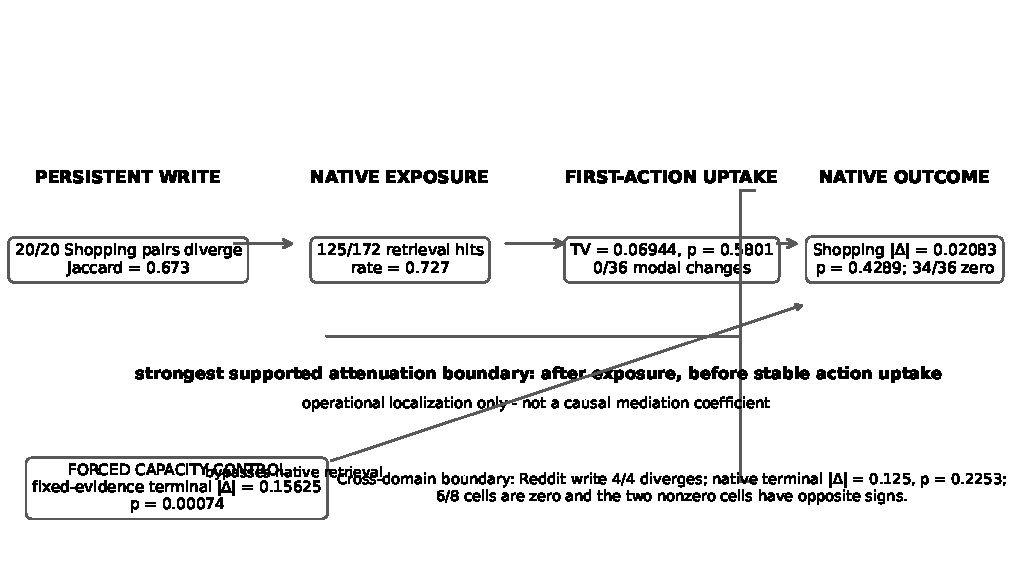
\includegraphics[width=\linewidth,trim=4pt 26pt 8pt 80pt,clip]{figures/fig4_stage_resolved_transport.pdf}
\caption{\textbf{Native transport and forced capacity are different experimental surfaces.} The horizontal path is the deployed reuse chain: persistent write $\rightarrow$ native source-item exposure $\rightarrow$ first-action uptake $\rightarrow$ native outcome. The forced fixed-evidence arm bypasses retrieval and is shown as a side capacity control. On the frozen Shopping tests, first-action uptake is the first unsupported measured native stage after write and item exposure are established; this is an evidence boundary, not a latent causal bottleneck or mediation coefficient.}
\label{fig:stage-transport}
\end{figure}

\subsection{Why the one-step reward-to-behavior story fails}
A one-step interpretation would take the 256 forced rollouts as evidence that ``reward error propagates to future behavior.'' The native measurements show why this is too coarse. Forced injection estimates leverage conditional on making a particular memory state available; native transport additionally depends on retrieval competition, context composition, and policy uptake. Indeed, coarsened views of the same frozen system disagree: write-only looks strongly affected, retrieval-only looks active, native endpoint-only looks nearly null, and forced-only shows leverage. The full stage signature reconciles these summaries rather than averaging them. The difference between $0.15625$ forced leverage and $0.02083$ native Shopping terminal transport is therefore not a scalar attenuation factor to divide or average; the two surfaces answer different questions.

Conversely, looking only at the native endpoint would also lose the mechanism: a $0.02083$ Shopping terminal difference does not tell us that the writer failed, that memory was unavailable, or that the downstream system was globally insensitive. The stage-resolved controls exclude or weaken each of those simpler accounts before the first-action boundary is reached.

The evaluation consequence is concrete. For a persistent update, report at least one state-change metric, one exposure measurement, and one downstream uptake/outcome metric; use a capacity control only if its bypassed stages are explicit. Where possible, distinguish source-item exposure from treatment-residual exposure rather than treating retrieval of a shared carrier item as proof that the causal residual was consumed. Then report the first measured stage where evidence for transport is no longer supported, while keeping stage-specific power and measurement semantics explicit, rather than crediting the update with behavioral authority because its representation changed or because a retrieved item appeared in context.
